% Build: cd paper && tectonic main.tex   (or: make)
% Template: IEEE conference. Swap \documentclass once the target venue is chosen.
\documentclass[conference]{IEEEtran}

\usepackage[utf8]{inputenc}
\usepackage{amsmath,amssymb}
\usepackage{graphicx}
\usepackage{booktabs}
\usepackage{xcolor}
\usepackage{tikz}
\usetikzlibrary{positioning,arrows.meta,shapes.geometric}
\usepackage[hidelinks]{hyperref}
\usepackage{cleveref}

\graphicspath{{figures/}}

\begin{document}

\title{Deterministic Safety Rules and Guideline Retrieval for Small Open-Source LLMs in Emergency Triage: An Ablation Study on MIMIC-IV-ED}

\author{\IEEEauthorblockN{Arjun Singh}
\IEEEauthorblockA{\textit{Affiliation TBD}}}

\maketitle

\begin{abstract}
TODO: write last. One sentence each: problem, gap, method, dataset, headline result, implication.
\end{abstract}

\begin{IEEEkeywords}
emergency triage, large language models, retrieval-augmented generation, clinical safety, MIMIC-IV-ED
\end{IEEEkeywords}

% !TEX root = ../main.tex
\section{Introduction}\label{sec:intro}
Prior work~\cite{gaberEvaluatingLargeLanguage2025}.  % placeholder cite to exercise the bib
% Motivation: ED overcrowding, under-triage harms, LLM promise and risk.
% Gap: prior MIMIC LLM-triage work (e.g., Gaber et al.) uses large commercial models without hard safety overrides.
% Contributions (bullet list): safety layer, ablation, small local models, guideline RAG.

% !TEX root = ../main.tex
\section{Related Work}\label{sec:related}
\subsection{LLMs for ESI Triage}
\subsection{Retrieval-Augmented Clinical Decision Support}
\subsection{Rule-Based and Hybrid Safety Guardrails}

% !TEX root = ../main.tex
\section{Method}\label{sec:method}
% !TEX root = ../main.tex
% Triage pipeline as implemented in apps/server/src/modules/triage/triage.engine.ts
\begin{figure}[t]
\centering
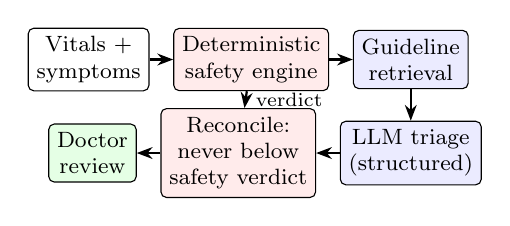
\begin{tikzpicture}[
  node distance=4mm and 3mm,
  box/.style={draw, rounded corners=2pt, align=center, font=\footnotesize, minimum height=7mm, inner sep=3pt},
  rule/.style={box, fill=red!8},
  llm/.style={box, fill=blue!8},
  human/.style={box, fill=green!10},
  arr/.style={-{Stealth[length=2mm]}, thick}
]
\node[box] (in) {Vitals +\\symptoms};
\node[rule, right=of in] (safe) {Deterministic\\safety engine};
\node[llm, right=of safe] (rag) {Guideline\\retrieval};
\node[llm, below=of rag] (llm) {LLM triage\\(structured)};
\node[rule, left=of llm] (rec) {Reconcile:\\never below\\safety verdict};
\node[human, left=of rec] (doc) {Doctor\\review};

\draw[arr] (in) -- (safe);
\draw[arr] (safe) -- (rag);
\draw[arr] (rag) -- (llm);
\draw[arr] (llm) -- (rec);
\draw[arr] (rec) -- (doc);
\draw[arr, dashed] (safe) -- node[right, font=\scriptsize] {verdict} (rec);
\end{tikzpicture}
\caption{JeevanSetu triage pipeline. Red: deterministic components; blue: LLM components; green: human-in-the-loop.}
\label{fig:pipeline}
\end{figure}

\subsection{Deterministic Safety Engine}
% Source: apps/server/src/modules/safety/safety.engine.ts
\subsection{Guideline Retrieval}
% Source: medical-pdf/ingestion/, apps/server/src/modules/rag/
\subsection{LLM Triage and Safety Reconciliation}
% Source: apps/server/src/modules/triage/triage.engine.ts, triage.prompts.ts

% !TEX root = ../main.tex
\section{Experimental Setup}\label{sec:experiments}
\subsection{Dataset}
% MIMIC-IV-ED cohort; ground truth = triage-nurse ESI (acuity field), not expert consensus.
\subsection{Ablation Configurations}
% (1) rules only, (2) LLM only, (3) LLM+RAG, (4) LLM+safety, (5) full.
\subsection{Models}
\subsection{Metrics}
% Exact accuracy, within-1 accuracy, under-triage (primary), over-triage, safety-rule precision, latency.

% !TEX root = ../main.tex
\section{Results}\label{sec:results}
% Every number here must come from a results file in the repo; note which one in a comment.

% !TEX root = ../main.tex
\section{Discussion}\label{sec:discussion}
\subsection{Limitations}

% !TEX root = ../main.tex
\section{Conclusion}\label{sec:conclusion}


\bibliographystyle{IEEEtran}
\bibliography{references}

\end{document}
